\documentclass[11pt]{article}
\usepackage[margin=1in]{geometry}
\usepackage{amsmath, amssymb, amsthm}
\usepackage{tikz}
\usetikzlibrary{arrows.meta, positioning, calc}
\usepackage{xcolor}
\usepackage{microtype}
\usepackage{booktabs}
\usepackage{hyperref}
\hypersetup{colorlinks=true, linkcolor=blue!50!black, urlcolor=blue!50!black}

\newcommand{\lca}{L}
\newcommand{\del}{\mathsf{del}}
\newcommand{\ins}{\mathsf{ins}}
\newcommand{\fold}{\mathsf{fold}}
\usepackage{pifont}

\tikzset{
  vtx/.style  ={draw, circle, minimum size=7.5mm, inner sep=0pt, fill=blue!8,  line width=0.6pt},
  rootv/.style={draw, circle, minimum size=7.5mm, inner sep=0pt, fill=black!12, line width=0.6pt, font=\bfseries},
  dead/.style ={draw, circle, minimum size=7.5mm, inner sep=0pt, densely dashed, fill=black!4, text=black!45},
  par/.style  ={-{Stealth[length=2.2mm]}, line width=0.7pt},
  rng/.style  ={|-|, line width=1.1pt},
  rngB/.style ={|-|, line width=1.1pt, blue!60!black},
  rngR/.style ={|-|, line width=1.1pt, red!70!black},
  lab/.style  ={font=\scriptsize, text=black!65},
  capt/.style ={font=\small\itshape, text=black!75},
}

\title{\bfseries The Delta Tree\\[2pt]
\large A tombstone-free replicated list with relative ranges, isometric
deletion,\\ and an identity-arbitrated merge}
\author{Sal / FP Launchpad --- KC + Claude}
\date{2026-07-14}

\begin{document}
\maketitle
\sloppy

\begin{abstract}
\noindent
This note gives the complete design of the \emph{delta tree}, a replicated
list (sequence MRDT). The state has two parts with strictly separated
roles. The \emph{rendering} is a tree of live nodes carrying
\emph{parent-relative} fractional ranges (deltas): reads are a geometric
traversal, inserts carve a slice of the anchor's free space, and delete is
an \emph{isometric fold} --- the dead node's fraction is composed into its
children's, so every survivor's displayed position is arithmetically
unchanged. The \emph{ledger} maps each identifier to its birth parent ---
written once, never mutated, never read outside merges. The merge
arbitrates all ordering from the ledger's immutable \emph{birth chains}
(the canonical order is the RGA order of the birth tree restricted to
survivors) and then re-derives the rendering; geometry is never an
arbiter. The design is machine-validated: clean on the full litmus battery
(L1--L25, the fooling probes, multi-epoch) except backward-run
interleaving (L19) --- the published RGA's own anomaly --- and clean on
420 randomized version-DAG executions. Stronger: a lockstep harness
asserting read-equality at every step shows the delta tree is
\emph{observationally equivalent to the published tombstoned RGA} on every
scenario and every random execution tried --- it admits exactly the North
Star's anomalies, while storing one immutable parent id per node in place
of tombstones in the sequence. Each design decision, in particular that
identity arbitrates and geometry only renders, is forced by a
machine-checked countermodel; \S\ref{sec:rationale} summarizes that
campaign and \S\ref{sec:mech} lays out the mechanization plan.
\end{abstract}

\section{The design}
\label{sec:design}

\paragraph{State.} $\sigma = (\rho, \Lambda)$.
The \emph{rendering} $\rho$ is a finite map over live nodes,
\[
  \rho : t \;\mapsto\; (\,\mathrm{par},\ (lo, hi),\ \mathrm{char}\,),
  \qquad 0 \le lo < hi \le 1 ,
\]
where timestamps $t$ double as element identities and $(lo,hi)$ is the
node's range \emph{relative to its parent's range} --- the \emph{delta}.
The root sentinel $0$ owns the unit interval and is never stored. A node's
\emph{absolute} range is the affine composition of the deltas along its
root path. The \emph{ledger} $\Lambda : t \mapsto \mathrm{birth\ parent}$
records each node's parent at birth --- written once at insert, never
mutated, retained through delete. Its entries are needed only while some
live node's birth chain passes through them (live-reachable scope), and
are prunable at causal stability. Reads never consult $\Lambda$; merges
never order by $\rho$.

\begin{figure}[h]
\centering
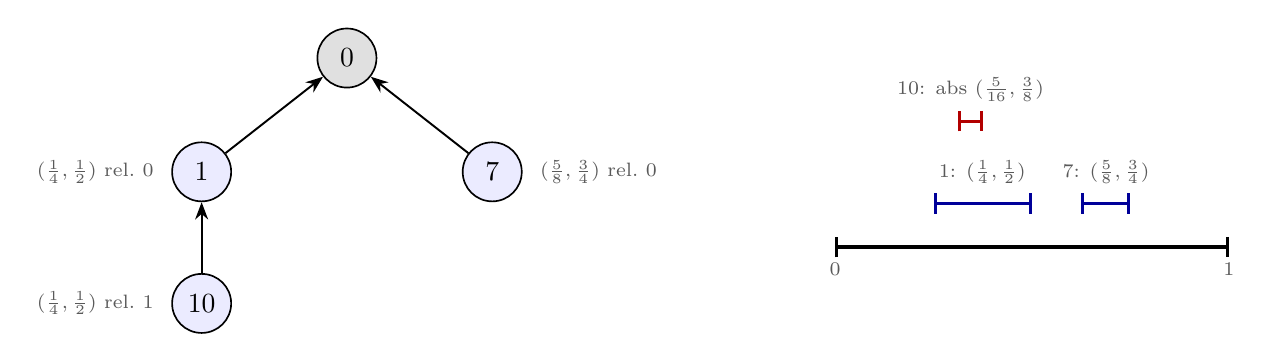
\begin{tikzpicture}[node distance=11mm]
  \node[rootv] (r) {$0$};
  \node[vtx, below left=9mm and 13mm of r] (a) {$1$};
  \node[vtx, below right=9mm and 13mm of r] (b) {$7$};
  \node[vtx, below=9mm of a] (c) {$10$};
  \draw[par] (a) -- (r); \draw[par] (b) -- (r); \draw[par] (c) -- (a);
  \node[lab, left=1mm of a]  {$(\tfrac14,\tfrac12)$ rel.\ $0$};
  \node[lab, right=1mm of b] {$(\tfrac58,\tfrac34)$ rel.\ $0$};
  \node[lab, left=1mm of c]  {$(\tfrac14,\tfrac12)$ rel.\ $1$};
  \begin{scope}[xshift=62mm, yshift=-24mm]
    \draw[rng] (0,0) -- (5,0);
    \node[lab, below] at (0,-0.08) {$0$}; \node[lab, below] at (5,-0.08) {$1$};
    \draw[rngB] (1.25,0.55) -- (2.5,0.55);  \node[lab] at (1.87,0.95) {$1$: $(\tfrac14,\tfrac12)$};
    \draw[rngB] (3.125,0.55) -- (3.75,0.55); \node[lab] at (3.44,0.95) {$7$: $(\tfrac58,\tfrac34)$};
    \draw[rngR] (1.5625,1.6) -- (1.875,1.6); \node[lab] at (1.72,2.0) {$10$: abs $(\tfrac{5}{16},\tfrac38)$};
  \end{scope}
\end{tikzpicture}
\caption{The rendering is a tree of deltas (left); absolute ranges are
composed down the path (right): $10$'s absolute range is
$\tfrac14 + \tfrac14\cdot(\tfrac14,\tfrac12) = (\tfrac{5}{16},\tfrac38)$.
Display order: depth-first, children by descending range --- newest first.
The ledger for this state is $\Lambda = \{1 \mapsto 0,\ 7 \mapsto 0,\
10 \mapsto 1\}$.}
\label{fig:state}
\end{figure}

\paragraph{Insert.} $\ins(x \leftarrow a)$: \emph{carve} --- the new child
of anchor $a$ takes a slice of $a$'s free child-space above the current
head. With remaining relative gap $(b,1)$ (where $b$ is the current head's
$hi$, or $0$), the newcomer takes
$\bigl(b+\tfrac{w}{4},\, b+\tfrac{w}{2}\bigr)$, $w = 1-b$, leaving room
above for future siblings and below for its own children. Newer siblings
sit higher; the display (descending) shows them first --- the RGA
convention, realized geometrically instead of by timestamp comparison at
read time. And one ledger write: $\Lambda[x] := a$.

\paragraph{Delete: the isometric fold.} $\del(d)$: remove $d$'s record
from $\rho$; re-parent each child to the grandparent with the dead node's
delta composed in: $c.\mathrm{frac} := d.\mathrm{frac} \circ
c.\mathrm{frac}$. Every survivor's absolute position is unchanged ---
\emph{delete-order preservation is an arithmetic identity}, where the flat
RGA's climb re-sorts (the $[b,a,c]\to[c,b]$ anomaly that started this
exploration) and the rose tree's splice needed sixteen thousand proof
lines it ultimately could not have. $\Lambda$ is untouched.

\begin{figure}[h]
\centering
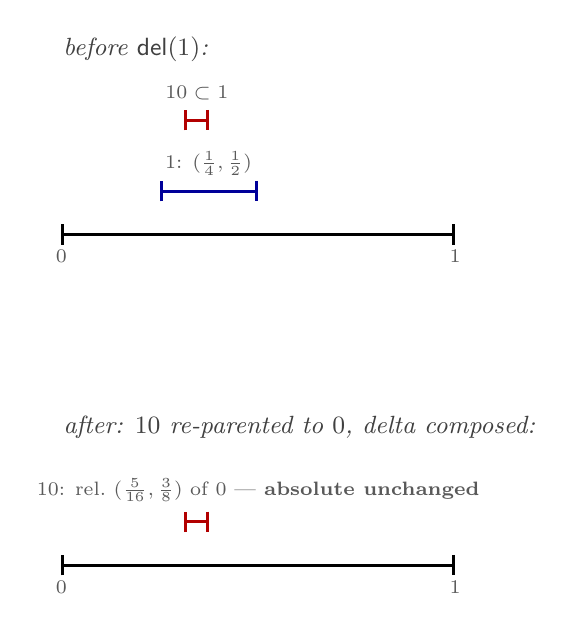
\begin{tikzpicture}
  \node[capt, anchor=west] at (-0.1,2.35) {before $\del(1)$:};
  \draw[rng] (0,0) -- (5,0);
  \node[lab, below] at (0,-0.08) {$0$}; \node[lab, below] at (5,-0.08) {$1$};
  \draw[rngB] (1.25,0.55) -- (2.5,0.55);  \node[lab] at (1.87,0.9) {$1$: $(\tfrac14,\tfrac12)$};
  \draw[rngR] (1.5625,1.45) -- (1.875,1.45); \node[lab] at (1.72,1.8) {$10 \subset 1$};
  \begin{scope}[yshift=-42mm]
  \node[capt, anchor=west] at (-0.1,1.75) {after: $10$ re-parented to $0$, delta composed:};
  \draw[rng] (0,0) -- (5,0);
  \node[lab, below] at (0,-0.08) {$0$}; \node[lab, below] at (5,-0.08) {$1$};
  \draw[rngR] (1.5625,0.55) -- (1.875,0.55);
  \node[lab] at (2.5,0.95) {$10$: rel.\ $(\tfrac{5}{16},\tfrac{3}{8})$ of $0$ --- \textbf{absolute unchanged}};
  \end{scope}
\end{tikzpicture}
\caption{The isometric fold. Deleting $1$ rewrites $10$'s delta to
$(\tfrac14,\tfrac12)\circ(\tfrac14,\tfrac12) = (\tfrac{5}{16},\tfrac38)$
relative to the root: the composition that \emph{was} its absolute range.
Nothing observable moves. $\Lambda$ still records $10 \mapsto 1$ --- the
identity of the dead parent survives in the ledger, and \S\ref{sec:merge}
is why it must.}
\label{fig:fold}
\end{figure}

\paragraph{Read.} Depth-first traversal of $\rho$, children by descending
range (newest first). Purely geometric; the ledger is never consulted.

\paragraph{The operation payload (per the proved RGA).} Following the
\emph{why-the-path-matters} analysis: $\mathsf{rc}$ must be
\textsf{Either} everywhere (any oriented insert/delete pair awakens the
refuted \texttt{cond\_comm\_base}), so the insert carries its anchor's
ancestor \emph{id-path} plus \textbf{one} absolute slice --- the composed
delta at mint time. Ids suffice for the path because the isometric fold
makes the absolute position invariant under ancestor deletion: a reordered
application resolves the id-path to the nearest live ancestor and
re-relativizes the carried absolute --- landing exactly where
insert-then-delete would have put it. On reachable states the anchor is
live and none of this is read: the path is ghost state in the strict,
machine-checked sense (\texttt{ins\_path\_free}).

\section{The merge}
\label{sec:merge}

The merge is built on three invariants; each is forced by a named
countermodel (\S\ref{sec:rationale}).

\begin{enumerate}
\item \textbf{Arbitration from identity only.} Every order decision at a
merge is computed from the ledger's immutable birth chains --- never from
current fractions, never by folding through mixed frames. Fractions drift:
merges re-derive them, and a repair inside one sibling family perturbs
numeric relations outside it. Chains never move, and a dead node's
timestamp persists in its descendants' chains, so every verdict it
participated in remains derivable, identically, at every replica and every
time.
\item \textbf{Geometry is a rendering.} The merge re-derives all fractions
to realize the canonical order. Between merges the geometry is
authoritative for \emph{display}; it is never authoritative for
\emph{arbitration}.
\item \textbf{Render/carve compatibility.} The re-render reproduces the
sequential carve's geometry --- oldest lowest, quarter slices, headroom
above --- so a post-merge state is indistinguishable from a sequentially
carved one and the next local carve behaves exactly as \S\ref{sec:design}
specifies. Merge output stays inside the image of the local operations.
\end{enumerate}

\noindent $\mathrm{merge}(\lca, A, B)$, $\lca$ the least common ancestor
(the LCA discipline guarantees common past $\subseteq \lca$):
\begin{enumerate}
  \item \emph{Ledger union}: $\Lambda' = \Lambda_\lca \cup \Lambda_A \cup
        \Lambda_B$. Entries are immutable, so the union is conflict-free.
  \item \emph{Survival} (OR-set): live iff in all three or born in exactly
        one branch.
  \item \emph{Live parent}: each survivor re-parents to its nearest
        surviving ancestor, found by walking $\Lambda'$ --- the fold's
        re-parenting, computed from identity instead of frames.
  \item \emph{Canonical order}: per live parent, children sort by their
        \textbf{birth chains} (root paths in the immutable birth tree):
        compare per level, newest timestamp first; an ancestor's chain is
        a prefix of its descendant's and sorts first. Equivalently:
        \emph{the canonical order is the RGA order of the birth tree,
        restricted to survivors}.
  \item \emph{Render}: re-derive all fractions realizing the canonical
        order by replaying the sequential carve --- children bottom-to-top,
        oldest first, each taking $(b + \tfrac{w}{4},\, b + \tfrac{w}{2})$,
        $w = 1 - b$ (invariant 3). Recurse.
\end{enumerate}

\paragraph{Worked example: concurrent twins.} $\lca$ empty; $A$:
$\ins(10\,{\leftarrow}\,0)$, $B$: $\ins(6\,{\leftarrow}\,0)$ --- identical
carves, identical slices $(\tfrac14,\tfrac12)$. Merge: chains are
$\langle 10 \rangle$ and $\langle 6 \rangle$; canonical order puts $10$
(newer) first. Render, oldest first: $6 \mapsto (\tfrac14,\tfrac12)$, then
$10$ above it with $w = \tfrac12$: $10 \mapsto (\tfrac58,\tfrac34)$.
Display $[10, 6]$ --- exactly the state a replica that saw $6$ then $10$
would have carved sequentially (invariant 3).

\paragraph{Worked example: a verdict surviving its arbiter's death.} The
scenario that kills every geometry-arbitrating alternative
(litmus L25), five nodes:

\begin{figure}[h]
\centering
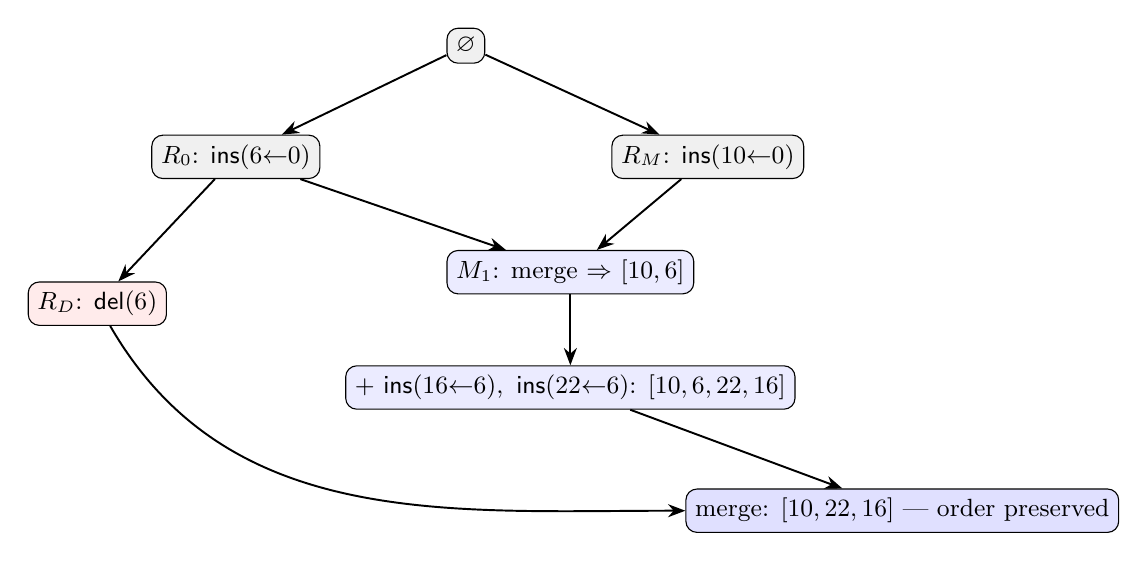
\begin{tikzpicture}[node distance=9mm and 16mm]
  \node[draw, rounded corners, fill=black!6, font=\small] (E)  {$\varnothing$};
  \node[draw, rounded corners, fill=black!6, font=\small, below left=of E]  (R0) {$R_0$: $\ins(6{\leftarrow}0)$};
  \node[draw, rounded corners, fill=black!6, font=\small, below right=of E] (RM) {$R_M$: $\ins(10{\leftarrow}0)$};
  \node[draw, rounded corners, fill=blue!8,  font=\small, below right=of R0] (M1) {$M_1$: merge $\Rightarrow$ $[10,6]$};
  \node[draw, rounded corners, fill=blue!8,  font=\small, below=of M1] (M1p) {$+\ \ins(16{\leftarrow}6),\ \ins(22{\leftarrow}6)$: $[10,6,22,16]$};
  \node[draw, rounded corners, fill=red!8,   font=\small, below left=13mm and -2mm of R0] (RD) {$R_D$: $\del(6)$};
  \node[draw, rounded corners, fill=blue!12, font=\small, below right=10mm and -14mm of M1p] (F) {merge: $[10,22,16]$ --- order preserved};
  \draw[par] (E) -- (R0); \draw[par] (E) -- (RM);
  \draw[par] (R0) -- (M1); \draw[par] (RM) -- (M1);
  \draw[par] (M1) -- (M1p);
  \draw[par] (R0) -- (RD);
  \draw[par] (M1p) -- (F); \draw[par] (RD) to[out=-60, in=180] (F);
\end{tikzpicture}
\caption{The $M_1$ merge ordered $10$ before $6$ (timestamps: $10>6$);
typing $22$ under $6$ co-displayed $10$ before $22$. The deleter branch
$R_D$ knew only $\{6\}$. At the final merge $6$ is dead --- yet the
verdict survives.}
\label{fig:l25}
\end{figure}

At the final merge the survivors are $\{10, 22, 16\}$, all with live
parent $0$. Their chains: $\langle 10 \rangle$ for the root-born $10$;
$\langle 6, 22 \rangle$ and $\langle 6, 16 \rangle$ for $6$'s heirs ---
the chains run \emph{through} the dead $6$. Comparing $10$ with $22$ at
the first level compares $10$ with $6$: the dead node's timestamp,
persisting in its heirs' chains, keeps deciding, and $10$ wins exactly as
$M_1$ ruled. Within $6$'s heirs, $22 > 16$ puts $22$ first. Display:
$[10, 22, 16]$ --- both previously co-displayed pairs preserved. Any
merge that instead orders by folded geometry lets $22$ re-litigate the
slot with its \emph{own} (newer) timestamp and win a contest its parent
had lost: the display flips to $[22, 10, 16]$.

\section{Design rationale: why identity arbitrates}
\label{sec:rationale}

Every choice above is the survivor of a machine-checked refutation
campaign over the ``geometric key'' design space (sixteen designs,
countermodels L17--L25 in \texttt{whiteboard/litmus/}; full record in its
\texttt{README} and this file's git history). In brief: eager scalar keys
die at the ceiling escapes (L17/L18); name-free carved ranges die at tie
inheritance (L20); re-ranging at merge dies at three-branch convergence
(L22); and a delta tree whose merge arbitrates from geometry while keeping
the state \emph{strictly} dead-free --- no dead identifier anywhere ---
dies at random-DAG scale by two mechanisms: \emph{fold-verdict erasure}
(a dead node's timestamp is load-bearing for repair verdicts it
participated in, and erasing it lets heirs re-litigate: the scenario of
fig.~\ref{fig:l25}) and \emph{repair non-locality} (re-slotting inside one
overlap family perturbs numeric relations outside it, so timestamp-decided
ties get re-decided by position at causally disjoint merges). Eight
variants of that family produced eight countermodels.

The campaign's summary is a triangle: of \{strictly dead-free, pairwise
display stability, topology convergence\}, every pairwise combination has
a machine-checked witness and the triple has only failed attempts ---
order verdicts must be re-derivable, identically, everywhere, and only
immutable data naming \emph{all} participants, including the dead ones,
guarantees it. The delta tree accepts the minimum toll the triangle
demands: one immutable parent id per node, at live-reachable scope, never
consulted by reads. The birth chains are precisely the one-sided immutable
path key (\texttt{path-2}'s after-side), stored as a parent pointer per
node instead of a materialized path; the delta tree is that
specification's runtime --- $O(1)$ isometric deletes and geometric reads
between merges. \emph{Identity for deciding, geometry for reading.}

\section{Validation}
\label{sec:validation}

\paragraph{The litmus battery.} The suite (\texttt{whiteboard/litmus/},
tests with provenance) ran the implementation
(\texttt{DeltaTreeV3} in \texttt{litmus/delta\_tree.py}).
``RGA$_\dagger$'' = the published, tombstoned RGA; ``RGA$_{tf}$'' = the
repo's \emph{proved} tombstone-free RGA.

\begin{center}\footnotesize
\begin{tabular}{@{}lccc l@{}}
\toprule
test & delta tree & RGA$_\dagger$ & RGA$_{tf}$ & what it detects \\
\midrule
L1 delete-reorder            & \checkmark & \checkmark & $\times$ & sequential splice re-sort \\
L2 splice fooling pair       & \checkmark & \checkmark & $\times$ & delete erases the side bit \\
L3a/b deep delete-runs       & \checkmark & \checkmark & \checkmark & transitive testimony loss \\
L4 criss-cross split         & \checkmark & \checkmark & \checkmark & the rose tree's refutation \\
L7 concurrent runs (g)       & \checkmark & \checkmark & \checkmark & forward interleaving \\
L17/L18 ceiling escapes      & \checkmark & \checkmark & \checkmark$/\times$ & eager-scalar staleness \\
L19 backward runs (h)        & $\times$   & $\times$   & $\times$ & prepend interleaving \\
L20 tie inheritance          & \checkmark & \checkmark & $\times$ & nameless carving \\
L21/L22/L23 topology         & \checkmark & \checkmark & \checkmark & re-ranging / frame leaks \\
L24 frame mixing             & \checkmark & \checkmark & \checkmark & cross-frame siblings \\
L25 fold-verdict inheritance & \checkmark & \checkmark & $\times$ & fig.~\ref{fig:l25}'s scenario \\
L5/L8--L13/L16 slot family   & \checkmark & \checkmark & $\times$ (L8/9/13) & w-slot / puncture family \\
M1 two epochs                & \checkmark & \checkmark & \checkmark & key exhaustion across merges \\
L14/L15 fooling probes       & \checkmark$^{\dagger}$ & \checkmark$^{\dagger}$ & $\times$ both & bounded-state impossibility \\
DAG PBT                      & \checkmark (120/120, 300/300) & \checkmark & $\times$ (80/120) & random branches and merges \\
\bottomrule
\end{tabular}
\end{center}

\noindent $^{\dagger}$\,the delta tree and RGA$_\dagger$ \emph{escape}
the impossibility probes the way the spine designs do: their retained data
(the ledger; the tombstones) distinguishes the probes' two worlds, so the
impossibility's bounded-state hypothesis does not apply.

\paragraph{The execution model.} Randomized version-DAG executions
(\texttt{litmus/pbt.py}): $n$ replicas; per round each replica either
issues honest operations against its own read or merges with a peer ---
legal only when some recorded version's event set equals the two heads'
intersection (the LCA discipline); final convergence rounds drive all
replicas to the full event set along different merge paths. Checks:
\textbf{FLIP} (global pairwise display stability: across every read of
every replica, no pair is ever shown in both orders), \textbf{CONV}
(equal event sets $\Rightarrow$ equal reads), \textbf{LIVE/DUP} (survival
correctness). Clean at 120/120 (4 replicas, 8 rounds) and 300/300
(6 replicas, 12 rounds), plus fresh-seed re-runs.

\paragraph{The anomaly contract, relative to the North Star.} What
anomalies does the delta tree admit, compared to the published
(tombstoned) RGA? The table shows column-for-column agreement; the true
statement is stronger. A lockstep harness (\texttt{PairedV3RGA} in
\texttt{delta\_tree.py}) runs both designs on identical histories and
asserts \emph{read equality at every apply, every merge, and every read}:
no divergence on any battery scenario --- the two designs' L19 failures
are the \emph{identical} interleaving --- nor on 420 randomized DAG
executions. \textbf{Empirically, the delta tree \emph{is} the published
RGA}, with the tombstones compacted out of the display structure into the
birth ledger: the canonical order (RGA order of the birth tree restricted
to survivors) is precisely what the tombstoned read computes when it
skips tombstones. The admitted anomalies are therefore exactly the North
Star's: backward-run (prepend) interleaving --- h, litmus L19, the
classic RGA weakness that motivated Fugue --- and nothing else;
strong-list (e) and oracle fidelity (f) hold on every scenario tested and
are unproven in general for both designs equally.

\section{Mechanization plan}
\label{sec:mech}

The two-part state suggests the proof structure directly.
\begin{itemize}
\item \textbf{Chains as the specification.} The canonical order is a
deterministic function of the event set (the birth tree is immutable;
survival is an OR-set), so convergence is determinism, and pairwise
display stability reduces to monotonicity of the canonical order under
event-set growth --- statements about immutable data, in the style of the
proved RGA's global-key re-sort.
\item \textbf{The rendering as a refinement.} The geometric layer owes
exactly invariants 2 and 3: the merge's render realizes the canonical
order, and its output is in the image of the local operations. Local
steps preserve the correspondence (the isometric fold is
position-invariant by construction).
\item \textbf{The conjectured headline theorem.}
$\mathrm{read}_{\text{delta}} = \mathrm{read}_{\mathrm{RGA}_\dagger}$ on
all histories --- the delta tree as a \emph{compaction} of the published
RGA, inheriting the North Star's specification wholesale. The lockstep
harness is this theorem's test double.
\item \textbf{Framework fit.} A Conditioned MRDT with $\mathsf{rc} =
\textsf{Either}$ everywhere and the id-path payload of
\S\ref{sec:design}, reusing the proved RGA's conditioning scaffolding
(honest delivery; born accuracy + applicable delivery).
\end{itemize}

\paragraph{Provenance.} Every table cell and number in this note is
reproduced by \texttt{whiteboard/litmus/}: \texttt{litmus.py} (the
battery), \texttt{pbt.py} (the execution model), \texttt{delta\_tree.py}
(\texttt{DeltaTreeV3}, the refuted geometry-arbitrating variants kept as
regression artifacts, the lockstep equivalence harness, and the self-test
runner). The refutation campaign that fixed this design's invariants is
recorded in \texttt{whiteboard/litmus/README.md} and in this file's git
history.

\end{document}
